% L04_mini10.tex -- Fintech Security and Regulation
% 10-Slide Arc: WHY > FEEL > WHAT > CASE > HOW > RISK > WHERE > IMPACT > SO WHAT > ACT
% Self-contained (no \input{} commands, no \includegraphics)
% Compile: pdflatex L04_mini10.tex (twice for overlays)
% ============================================================

\documentclass[aspectratio=169, 11pt]{beamer}
\usetheme{Madrid}
\usecolortheme{whale}
\usepackage{tikz,pgfplots,booktabs,multicol,amsmath,graphicx,hyperref,xcolor}
\usetikzlibrary{arrows.meta,positioning,shapes.geometric,calc,decorations.pathmorphing}
\pgfplotsset{compat=1.18}

% ---- Colour palette ----------------------------------------
\definecolor{mlpurple}{HTML}{9467BD}
\definecolor{mlblue}{HTML}{1F77B4}
\definecolor{mlred}{HTML}{D62728}
\definecolor{mlorange}{HTML}{FF7F0E}
\definecolor{mlgreen}{HTML}{2CA02C}
\definecolor{mlgray}{HTML}{7F7F7F}
\definecolor{mlteal}{HTML}{0D7377}
\definecolor{mlcyan}{HTML}{14BDEB}

% ---- Beamer theme overrides --------------------------------
\setbeamercolor{structure}{fg=mlteal}
\setbeamercolor{palette primary}{bg=mlteal,fg=white}
\setbeamercolor{palette secondary}{bg=mlteal!80,fg=white}
\setbeamercolor{palette tertiary}{bg=mlteal!60,fg=white}
\setbeamercolor{palette quaternary}{bg=mlteal,fg=white}
\setbeamercolor{frametitle}{bg=mlteal!10,fg=mlteal}
\setbeamercolor{title}{fg=white}
\setbeamercolor{subtitle}{fg=mlcyan}
\setbeamercolor{block title}{bg=mlteal,fg=white}
\setbeamercolor{block body}{bg=mlteal!8,fg=black}
\setbeamercolor{block title alerted}{bg=mlred,fg=white}
\setbeamercolor{block body alerted}{bg=mlred!8,fg=black}
\setbeamercolor{block title example}{bg=mlgreen,fg=white}
\setbeamercolor{block body example}{bg=mlgreen!8,fg=black}
\setbeamerfont{frametitle}{size=\large,series=\bfseries}

% ---- Bottom note command -----------------------------------
\newcommand{\bottomnote}[1]{%
  \vfill
  \begin{beamercolorbox}[wd=\textwidth,ht=2ex,dp=1ex]{palette primary}
    \tiny\hspace{1em}#1
  \end{beamercolorbox}}

% ---- Metadata ----------------------------------------------
\title{Fintech Security and Regulation}
\subtitle{10-Slide Mini Lecture}
\author{Joerg Osterrieder}
\institute{University of Zurich}
\date{Spring 2026}
\setbeamertemplate{navigation symbols}{}
\graphicspath{{}}

% ============================================================
\begin{document}
% ============================================================

% TITLE FRAME (not counted in the 10)
\begin{frame}
  \titlepage
\end{frame}

% ============================================================
%  FRAME 1 -- WHY: TikZ comic -- compliance officer drowning
%             in stacked regulation documents, drone "RegTech"
% ============================================================
\begin{frame}{Why RegTech? The Compliance Tsunami}
\begin{center}
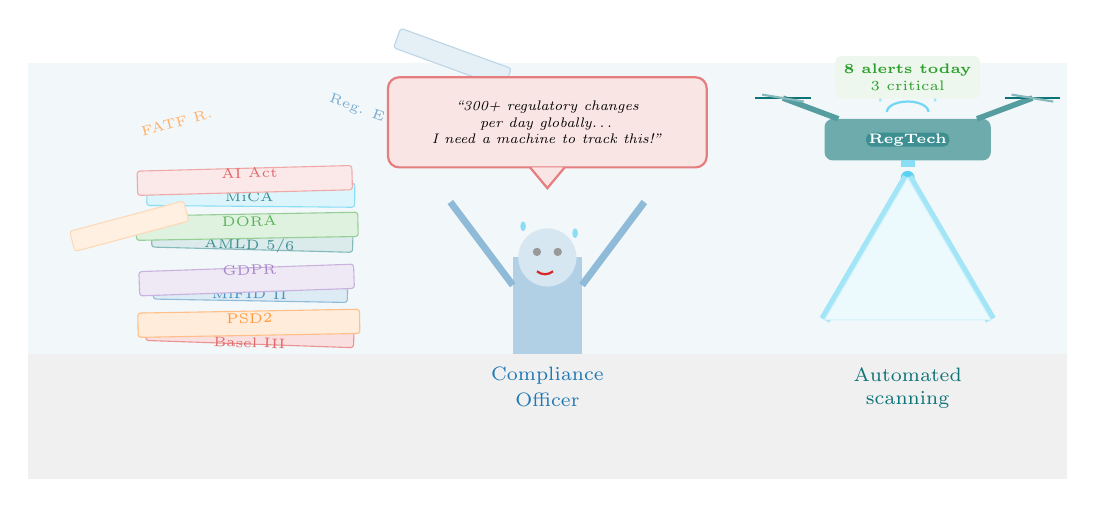
\begin{tikzpicture}[scale=0.88]

  % ---- Floor / background ------------------------------------
  \fill[mlgray!12] (-7.5,-1.8) rectangle (7.5,0.0);
  \fill[mlblue!6]  (-7.5, 0.0) rectangle (7.5,4.2);

  % ============================================================
  %  LEFT SIDE: Stacked regulation documents
  % ============================================================
  % Document stack (bottom to top, increasingly tilted)
  \fill[mlred!15,draw=mlred!50,rounded corners=1pt,rotate=-2]
    (-5.8,0.0) rectangle (-2.8,0.35);
  \node[font=\tiny,text=mlred!70,rotate=-2] at (-4.3,0.17) {Basel III};

  \fill[mlorange!15,draw=mlorange!50,rounded corners=1pt,rotate=1]
    (-5.9,0.35) rectangle (-2.7,0.70);
  \node[font=\tiny,text=mlorange!80,rotate=1] at (-4.3,0.52) {PSD2};

  \fill[mlblue!15,draw=mlblue!50,rounded corners=1pt,rotate=-1]
    (-5.7,0.70) rectangle (-2.9,1.05);
  \node[font=\tiny,text=mlblue!80,rotate=-1] at (-4.3,0.87) {MiFID II};

  \fill[mlpurple!15,draw=mlpurple!50,rounded corners=1pt,rotate=2]
    (-5.85,1.05) rectangle (-2.75,1.40);
  \node[font=\tiny,text=mlpurple!80,rotate=2] at (-4.3,1.22) {GDPR};

  \fill[mlteal!15,draw=mlteal!50,rounded corners=1pt,rotate=-1.5]
    (-5.75,1.40) rectangle (-2.85,1.75);
  \node[font=\tiny,text=mlteal!80,rotate=-1.5] at (-4.3,1.57) {AMLD 5/6};

  \fill[mlgreen!15,draw=mlgreen!50,rounded corners=1pt,rotate=1]
    (-5.9,1.75) rectangle (-2.7,2.10);
  \node[font=\tiny,text=mlgreen!80,rotate=1] at (-4.3,1.92) {DORA};

  \fill[mlcyan!15,draw=mlcyan!50,rounded corners=1pt,rotate=-0.5]
    (-5.8,2.10) rectangle (-2.8,2.45);
  \node[font=\tiny,text=mlteal!80,rotate=-0.5] at (-4.3,2.27) {MiCA};

  \fill[mlred!10,draw=mlred!40,rounded corners=1pt,rotate=1.5]
    (-5.85,2.45) rectangle (-2.75,2.80);
  \node[font=\tiny,text=mlred!70,rotate=1.5] at (-4.3,2.62) {AI Act};

  % More documents raining down
  \fill[mlorange!12,draw=mlorange!30,rounded corners=1pt,rotate=15]
    (-6.2,3.2) rectangle (-4.5,3.5);
  \node[font=\tiny,text=mlorange!60,rotate=15] at (-5.35,3.35) {FATF R.};
  \fill[mlblue!12,draw=mlblue!30,rounded corners=1pt,rotate=-20]
    (-3.6,3.4) rectangle (-1.9,3.7);
  \node[font=\tiny,text=mlblue!60,rotate=-20] at (-2.75,3.55) {Reg. E};

  % ============================================================
  %  CENTRE: Compliance officer drowning
  % ============================================================
  % Body (partially submerged in documents)
  \fill[mlblue!35] (-0.5,0.0) rectangle (0.5,1.4);
  % Head
  \fill[mlblue!18] (0.0,1.4) circle (0.42);
  % Worried eyes
  \fill[mlgray!80] (-0.15,1.48) circle (0.06);
  \fill[mlgray!80] ( 0.15,1.48) circle (0.06);
  % Worried mouth
  \draw[mlred,thick] (-0.15,1.20) arc(230:310:0.18);
  % Arms raised in distress
  \draw[mlblue!50,line width=2.5pt] (-0.5,1.0) -- (-1.4,2.2);
  \draw[mlblue!50,line width=2.5pt] ( 0.5,1.0) -- ( 1.4,2.2);
  % Sweat drops
  \fill[mlcyan!50] (-0.35,1.85) ellipse (0.04 and 0.07);
  \fill[mlcyan!50] ( 0.40,1.75) ellipse (0.04 and 0.07);
  % Label
  \node[font=\scriptsize,text=mlblue] at (0.0,-0.30) {Compliance};
  \node[font=\scriptsize,text=mlblue] at (0.0,-0.65) {Officer};

  % Speech bubble
  \fill[mlred!12,rounded corners=4pt] (-2.3,2.7) rectangle (2.3,4.0);
  \draw[mlred!60,thick,rounded corners=4pt] (-2.3,2.7) rectangle (2.3,4.0);
  \fill[mlred!12] (-0.25,2.7) -- (0.0,2.4) -- (0.25,2.7) -- cycle;
  \draw[mlred!60,thick] (-0.25,2.7) -- (0.0,2.4) -- (0.25,2.7);
  \node[font=\tiny,text width=4.2cm,align=center] at (0.0,3.35)
    {\textit{``300+ regulatory changes}\\
     \textit{per day globally\ldots}\\
     \textit{I need a machine to track this!''}};

  % ============================================================
  %  RIGHT SIDE: RegTech drone hovering above
  % ============================================================
  % Drone body
  \fill[mlteal!60,rounded corners=3pt] (4.0,2.8) rectangle (6.4,3.4);
  \fill[mlteal!80,rounded corners=2pt] (4.6,3.0) rectangle (5.8,3.2);
  % Rotor arms
  \draw[mlteal!70,line width=2pt] (4.2,3.4) -- (3.4,3.7);
  \draw[mlteal!70,line width=2pt] (6.2,3.4) -- (7.0,3.7);
  % Rotor blades (spinning arcs)
  \draw[mlteal,thick] (3.0,3.7) -- (3.8,3.7);
  \draw[mlteal!50,thick] (3.1,3.75) -- (3.7,3.65);
  \draw[mlteal,thick] (6.6,3.7) -- (7.4,3.7);
  \draw[mlteal!50,thick] (6.7,3.75) -- (7.3,3.65);
  % Camera / sensor underneath
  \fill[mlcyan!50] (5.1,2.7) rectangle (5.3,2.8);
  \fill[mlcyan!70] (5.2,2.55) circle (0.10);
  % Label on drone body
  \node[font=\tiny\bfseries,text=white] at (5.2,3.1) {RegTech};
  % Scanning beam
  \draw[mlcyan!40,line width=4pt] (5.2,2.55) -- (4.0,0.5);
  \draw[mlcyan!40,line width=4pt] (5.2,2.55) -- (6.4,0.5);
  \draw[mlcyan!20,fill=mlcyan!8] (4.0,0.5) -- (5.2,2.55) -- (6.4,0.5) -- cycle;
  % Signal waves from drone
  \draw[mlcyan!60,thick] (5.5,3.5) arc(0:180:0.3 and 0.15);
  \draw[mlcyan!40,thick] (5.6,3.65) arc(0:180:0.4 and 0.20);
  % Ground label
  \node[font=\scriptsize,text=mlteal] at (5.2,-0.30) {Automated};
  \node[font=\scriptsize,text=mlteal] at (5.2,-0.65) {scanning};
  % Drone speech
  \node[font=\tiny,text=mlgreen,align=center,
        fill=mlgreen!8,rounded corners=2pt,inner sep=3pt]
    at (5.2,4.0) {\textbf{8 alerts today}\\3 critical};

\end{tikzpicture}
\end{center}
\bottomnote{Slide 1/10 --- WHY | Financial Technology -- MSc | University of Zurich | Spring 2026}
\end{frame}

% ============================================================
%  FRAME 2 -- FEEL: Text prompt -- compliance rules count
% ============================================================
\begin{frame}{A Moment of Reflection: How Many Rules?}

\vspace{0.2em}
\begin{block}{The Invisible Regulatory Web}
\small Regulation is the air that finance breathes: invisible until it chokes you.
Before we analyse the system, estimate the compliance burden you interact with every day.
\end{block}

\vspace{0.3em}
\small Think about a single banking relationship you hold. Consider:

\vspace{0.15em}
\begin{columns}[T]
\begin{column}{0.48\textwidth}
\begin{itemize}\small
  \item[\textcolor{mlteal}{\textbullet}] \textbf{Onboarding:} How many documents did you submit to open the account?
  \item[\textcolor{mlteal}{\textbullet}] \textbf{Monitoring:} Has your bank ever flagged or blocked a transaction?
  \item[\textcolor{mlteal}{\textbullet}] \textbf{Privacy:} How many consent forms did you sign (GDPR, data sharing)?
\end{itemize}
\end{column}
\begin{column}{0.48\textwidth}
\begin{itemize}\small
  \item[\textcolor{mlcyan}{\textbullet}] \textbf{Cross-border:} Were you asked extra questions for international transfers?
  \item[\textcolor{mlcyan}{\textbullet}] \textbf{Limits:} Do you have daily transfer caps you never requested?
  \item[\textcolor{mlcyan}{\textbullet}] \textbf{Reporting:} Has your bank mentioned ``suspicious activity'' obligations?
\end{itemize}
\end{column}
\end{columns}

\vspace{0.3em}
\begin{exampleblock}{Quick Estimate}
\small How many compliance rules does your bank follow? \textbf{Hint: thousands.}
A large global bank tracks over \textbf{200 regulatory bodies} across 60+ jurisdictions, adapting to an average of \textbf{300 regulatory changes per business day}. Every one of those rules ultimately touches your account.
\end{exampleblock}

\bottomnote{Slide 2/10 --- FEEL | Financial Technology -- MSc | University of Zurich | Spring 2026}
\end{frame}

% ============================================================
%  FRAME 3 -- WHAT: Table -- regulatory approaches by jurisdiction
% ============================================================
\begin{frame}{What Are the Regulatory Approaches? Five Jurisdictions Compared}

\vspace{0.1em}
\begin{center}
\scriptsize
\begin{tabular}{@{}p{2.0cm}p{2.2cm}p{2.2cm}p{2.2cm}p{2.2cm}p{2.2cm}@{}}
\toprule
\textbf{Dimension} & \textbf{United States} & \textbf{European Union} & \textbf{United Kingdom} & \textbf{Singapore} & \textbf{China} \\
\midrule
\textbf{Philosophy} & Activity-based, fragmented & Precautionary, harmonised & Innovation-friendly, principles-based & Risk-proportionate, sandbox-first & State-directed, top-down \\[3pt]
\textbf{Sandbox} & \textcolor{mlred}{\textbf{Limited}} (state-level) & \textcolor{mlorange}{\textbf{Emerging}} (EBA/EIOPA) & \textcolor{mlgreen}{\textbf{Pioneer}} (FCA since 2016) & \textcolor{mlgreen}{\textbf{Strong}} (MAS FinTech) & \textcolor{mlorange}{\textbf{Selective}} (PBOC pilots) \\[3pt]
\textbf{Crypto stance} & \textcolor{mlorange}{\textbf{Unclear}}, SEC vs CFTC & \textcolor{mlgreen}{\textbf{MiCA}} (2024) & \textcolor{mlgreen}{\textbf{FCA regime}} evolving & \textcolor{mlgreen}{\textbf{PSA licensed}} & \textcolor{mlred}{\textbf{Banned}} (trading) \\[3pt]
\textbf{AML rigor} & \textcolor{mlgreen}{\textbf{BSA/OFAC}} strong & \textcolor{mlgreen}{\textbf{AMLD 6}} strict & \textcolor{mlgreen}{\textbf{MLR 2022}} robust & \textcolor{mlgreen}{\textbf{FATF-aligned}} & \textcolor{mlgreen}{\textbf{PBOC}} centralized \\[3pt]
\textbf{Data privacy} & Sectoral (CCPA, HIPAA) & \textcolor{mlgreen}{\textbf{GDPR}} gold standard & UK GDPR + DPA 2018 & PDPA 2012 & PIPL 2021 \\[3pt]
\textbf{Open banking} & \textcolor{mlred}{\textbf{Market-led}} (slow) & \textcolor{mlgreen}{\textbf{PSD2/PSD3}} mandated & \textcolor{mlgreen}{\textbf{CMA Order}} mandated & \textcolor{mlorange}{\textbf{API guidelines}} & \textcolor{mlred}{\textbf{State platforms}} \\[3pt]
\textbf{Key regulator(s)} & SEC, CFTC, OCC, FinCEN & EBA, ECB, ESMA & FCA, PRA, BOE & MAS & PBOC, CBIRC, CSRC \\
\bottomrule
\end{tabular}
\end{center}

\vspace{0.05em}
\begin{block}{No One-Size-Fits-All}
\scriptsize Innovation-friendly regimes (UK, Singapore) attract fintech HQs. Precautionary regimes (EU) provide consumer certainty. Fragmented regimes (US) create arbitrage. State-directed regimes (China) move fast but limit private innovation.
\end{block}

\bottomnote{Slide 3/10 --- WHAT | Financial Technology -- MSc | University of Zurich | Spring 2026}
\end{frame}

% ============================================================
%  FRAME 4 -- CASE: TikZ diagram -- money laundering
%             three-stage flow (placement -> layering -> integration)
% ============================================================
\begin{frame}{Case Study: The Three Stages of Money Laundering}
\begin{center}
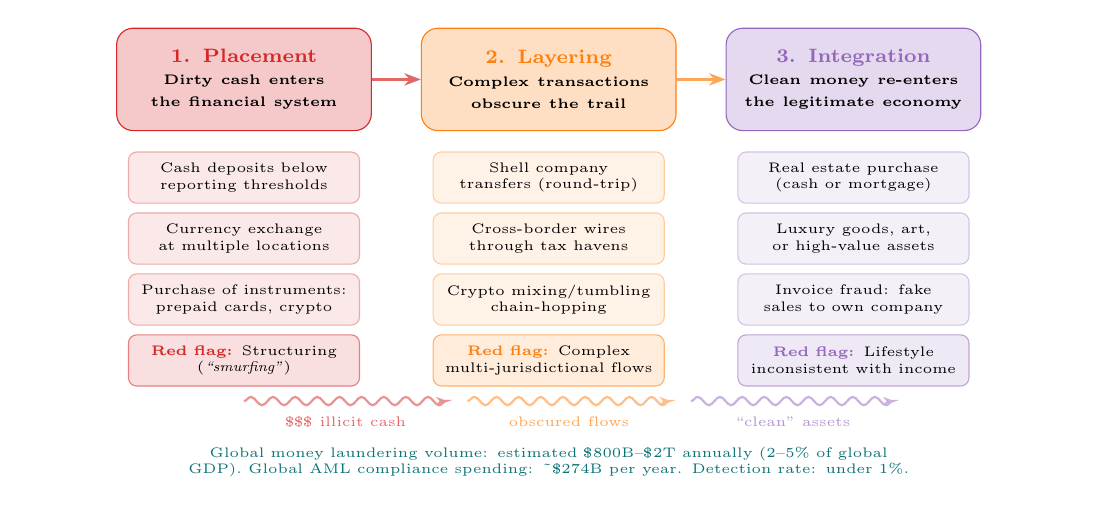
\begin{tikzpicture}[scale=0.86,
  stage/.style={rectangle,rounded corners=6pt,minimum width=3.2cm,
                minimum height=1.3cm,font=\scriptsize\bfseries,
                text centered,text width=3.0cm},
  detail/.style={rectangle,rounded corners=3pt,minimum width=2.8cm,
               minimum height=0.65cm,font=\tiny,
               text centered,text width=2.7cm},
  arr/.style={-{Stealth[length=6pt]},thick,mlgray!70},
  lbl/.style={font=\tiny\itshape,text=mlgray,midway}
]

  % ---- Stage headers (top row) --------------------------------
  \node[stage,fill=mlred!25,draw=mlred] (P) at (-4.5, 2.4)
    {\textcolor{mlred}{1. Placement}\\[2pt]
     \tiny Dirty cash enters\\the financial system};
  \node[stage,fill=mlorange!25,draw=mlorange] (L) at (0.0, 2.4)
    {\textcolor{mlorange}{2. Layering}\\[2pt]
     \tiny Complex transactions\\obscure the trail};
  \node[stage,fill=mlpurple!25,draw=mlpurple] (I) at (4.5, 2.4)
    {\textcolor{mlpurple}{3. Integration}\\[2pt]
     \tiny Clean money re-enters\\the legitimate economy};

  % Arrows between stages
  \draw[arr,mlred!70] (P.east) -- (L.west);
  \draw[arr,mlorange!70] (L.east) -- (I.west);

  % ---- Detail boxes under Placement ----------------------------
  \node[detail,fill=mlred!10,draw=mlred!40] at (-4.5, 0.95)
    {Cash deposits below\\reporting thresholds};
  \node[detail,fill=mlred!10,draw=mlred!40] at (-4.5, 0.05)
    {Currency exchange\\at multiple locations};
  \node[detail,fill=mlred!10,draw=mlred!40] at (-4.5,-0.85)
    {Purchase of instruments:\\prepaid cards, crypto};
  \node[detail,fill=mlred!15,draw=mlred!60] at (-4.5,-1.75)
    {\textcolor{mlred}{\textbf{Red flag:}} Structuring\\(\textit{``smurfing''})};

  % ---- Detail boxes under Layering -----------------------------
  \node[detail,fill=mlorange!10,draw=mlorange!40] at (0.0, 0.95)
    {Shell company\\transfers (round-trip)};
  \node[detail,fill=mlorange!10,draw=mlorange!40] at (0.0, 0.05)
    {Cross-border wires\\through tax havens};
  \node[detail,fill=mlorange!10,draw=mlorange!40] at (0.0,-0.85)
    {Crypto mixing/tumbling\\chain-hopping};
  \node[detail,fill=mlorange!15,draw=mlorange!60] at (0.0,-1.75)
    {\textcolor{mlorange}{\textbf{Red flag:}} Complex\\multi-jurisdictional flows};

  % ---- Detail boxes under Integration --------------------------
  \node[detail,fill=mlpurple!10,draw=mlpurple!40] at (4.5, 0.95)
    {Real estate purchase\\(cash or mortgage)};
  \node[detail,fill=mlpurple!10,draw=mlpurple!40] at (4.5, 0.05)
    {Luxury goods, art,\\or high-value assets};
  \node[detail,fill=mlpurple!10,draw=mlpurple!40] at (4.5,-0.85)
    {Invoice fraud: fake\\sales to own company};
  \node[detail,fill=mlpurple!15,draw=mlpurple!60] at (4.5,-1.75)
    {\textcolor{mlpurple}{\textbf{Red flag:}} Lifestyle\\inconsistent with income};

  % ---- Dollar flow arrows beneath stages -----------------------
  \draw[mlred!50,-{Stealth[length=4pt]},thick,decorate,
        decoration={snake,amplitude=1.5pt,segment length=8pt}]
    (-4.5,-2.35) -- (-1.5,-2.35);
  \node[font=\tiny,text=mlred!70] at (-3.0,-2.65) {\$\$\$ illicit cash};

  \draw[mlorange!50,-{Stealth[length=4pt]},thick,decorate,
        decoration={snake,amplitude=1.5pt,segment length=8pt}]
    (-1.2,-2.35) -- (1.8,-2.35);
  \node[font=\tiny,text=mlorange!70] at (0.3,-2.65) {obscured flows};

  \draw[mlpurple!50,-{Stealth[length=4pt]},thick,decorate,
        decoration={snake,amplitude=1.5pt,segment length=8pt}]
    (2.1,-2.35) -- (5.1,-2.35);
  \node[font=\tiny,text=mlpurple!70] at (3.6,-2.65) {``clean'' assets};

  % ---- Global AML cost note -----------------------------------
  \node[font=\tiny,text=mlteal,align=center,text width=13cm]
    at (0,-3.25)
    {Global money laundering volume: estimated \$800B--\$2T annually (2--5\% of global GDP).
     Global AML compliance spending: \textasciitilde\$274B per year. Detection rate: under 1\%.};

\end{tikzpicture}
\end{center}
\bottomnote{Slide 4/10 --- CASE | Financial Technology -- MSc | University of Zurich | Spring 2026}
\end{frame}

% ============================================================
%  FRAME 5 -- HOW: TikZ flow -- KYC process lifecycle
%             (application -> verification -> screening -> monitoring)
% ============================================================
\begin{frame}{How KYC Works: The Customer Lifecycle}
\begin{center}
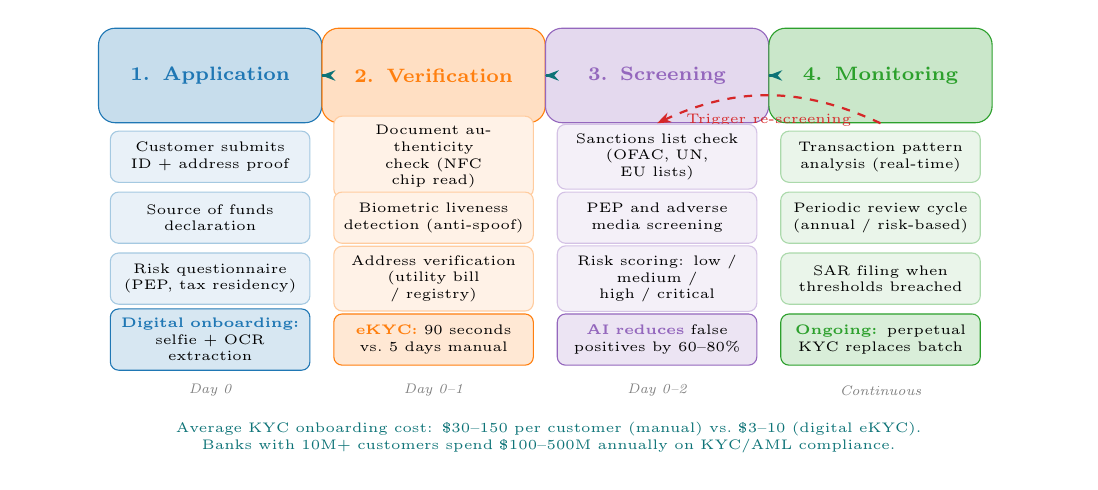
\begin{tikzpicture}[scale=0.86,
  phase/.style={rectangle,rounded corners=6pt,minimum width=2.7cm,
                minimum height=1.2cm,font=\scriptsize\bfseries,
                text centered,text width=2.6cm},
  stepbox/.style={rectangle,rounded corners=3pt,minimum width=2.4cm,
               minimum height=0.65cm,font=\tiny,
               text centered,text width=2.3cm},
  arr/.style={-{Stealth[length=5pt]},thick,mlteal},
  time/.style={font=\tiny\itshape,text=mlgray}
]

  % ---- Phase headers (top row) --------------------------------
  \node[phase,fill=mlblue!25,draw=mlblue]    (A) at (-5.0, 2.2)
    {\textcolor{mlblue}{1. Application}};
  \node[phase,fill=mlorange!25,draw=mlorange] (B) at (-1.7, 2.2)
    {\textcolor{mlorange}{2. Verification}};
  \node[phase,fill=mlpurple!25,draw=mlpurple]  (C) at (1.6, 2.2)
    {\textcolor{mlpurple}{3. Screening}};
  \node[phase,fill=mlgreen!25,draw=mlgreen]  (D) at (4.9, 2.2)
    {\textcolor{mlgreen}{4. Monitoring}};

  % Arrows between phases
  \draw[arr] (A.east) -- (B.west);
  \draw[arr] (B.east) -- (C.west);
  \draw[arr] (C.east) -- (D.west);

  % Feedback loop from Monitoring back to Screening
  \draw[arr,mlred,dashed,bend right=25]
    (D.south) to node[font=\tiny,text=mlred,below,yshift=-3pt]{Trigger re-screening} (C.south);

  % ---- Step boxes under Application ----------------------------
  \node[stepbox,fill=mlblue!10,draw=mlblue!40]  at (-5.0, 1.0)
    {Customer submits\\ID + address proof};
  \node[stepbox,fill=mlblue!10,draw=mlblue!40]  at (-5.0, 0.1)
    {Source of funds\\declaration};
  \node[stepbox,fill=mlblue!10,draw=mlblue!40]  at (-5.0,-0.8)
    {Risk questionnaire\\(PEP, tax residency)};
  \node[stepbox,fill=mlblue!18,draw=mlblue]     at (-5.0,-1.7)
    {\textcolor{mlblue}{\textbf{Digital onboarding:}}\\selfie + OCR extraction};

  \node[time] at (-5.0,-2.45) {Day 0};

  % ---- Step boxes under Verification --------------------------
  \node[stepbox,fill=mlorange!10,draw=mlorange!40] at (-1.7, 1.0)
    {Document authenticity\\check (NFC chip read)};
  \node[stepbox,fill=mlorange!10,draw=mlorange!40] at (-1.7, 0.1)
    {Biometric liveness\\detection (anti-spoof)};
  \node[stepbox,fill=mlorange!10,draw=mlorange!40] at (-1.7,-0.8)
    {Address verification\\(utility bill / registry)};
  \node[stepbox,fill=mlorange!18,draw=mlorange]    at (-1.7,-1.7)
    {\textcolor{mlorange}{\textbf{eKYC:}} 90 seconds\\vs.\ 5 days manual};

  \node[time] at (-1.7,-2.45) {Day 0--1};

  % ---- Step boxes under Screening ------------------------------
  \node[stepbox,fill=mlpurple!10,draw=mlpurple!40] at (1.6, 1.0)
    {Sanctions list check\\(OFAC, UN, EU lists)};
  \node[stepbox,fill=mlpurple!10,draw=mlpurple!40] at (1.6, 0.1)
    {PEP and adverse\\media screening};
  \node[stepbox,fill=mlpurple!10,draw=mlpurple!40] at (1.6,-0.8)
    {Risk scoring: low /\\medium / high / critical};
  \node[stepbox,fill=mlpurple!18,draw=mlpurple]    at (1.6,-1.7)
    {\textcolor{mlpurple}{\textbf{AI reduces}} false\\positives by 60--80\%};

  \node[time] at (1.6,-2.45) {Day 0--2};

  % ---- Step boxes under Monitoring -----------------------------
  \node[stepbox,fill=mlgreen!10,draw=mlgreen!40] at (4.9, 1.0)
    {Transaction pattern\\analysis (real-time)};
  \node[stepbox,fill=mlgreen!10,draw=mlgreen!40] at (4.9, 0.1)
    {Periodic review cycle\\(annual / risk-based)};
  \node[stepbox,fill=mlgreen!10,draw=mlgreen!40] at (4.9,-0.8)
    {SAR filing when\\thresholds breached};
  \node[stepbox,fill=mlgreen!18,draw=mlgreen]    at (4.9,-1.7)
    {\textcolor{mlgreen}{\textbf{Ongoing:}} perpetual\\KYC replaces batch};

  \node[time] at (4.9,-2.45) {Continuous};

  % ---- Bottom note on cost ------------------------------------
  \node[font=\tiny,text=mlteal,align=center,text width=13cm]
    at (0,-3.15)
    {Average KYC onboarding cost: \$30--150 per customer (manual) vs.\ \$3--10 (digital eKYC).
     Banks with 10M+ customers spend \$100--500M annually on KYC/AML compliance.};

\end{tikzpicture}
\end{center}
\bottomnote{Slide 5/10 --- HOW | Financial Technology -- MSc | University of Zurich | Spring 2026}
\end{frame}

% ============================================================
%  FRAME 6 -- RISK: TikZ comic -- fintech startup looking
%             at map with 50 different license requirements
% ============================================================
\begin{frame}{The Licensing Labyrinth: A Startup's Nightmare}
\begin{columns}[T]
\begin{column}{0.52\textwidth}
\vspace{0.2em}
\begin{center}
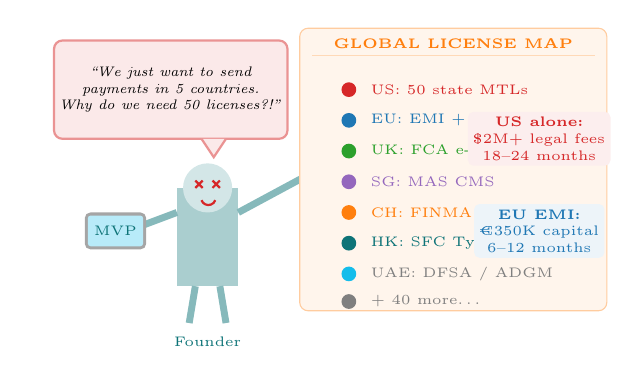
\begin{tikzpicture}[scale=0.78]

  % ---- Startup founder figure ----------------------------------
  % Body
  \fill[mlteal!35] (-0.5,-0.4) rectangle (0.5,1.2);
  % Head
  \fill[mlteal!18] (0.0,1.2) circle (0.40);
  % Confused eyes (X shapes)
  \draw[mlred,thick] (-0.2,1.32) -- (-0.08,1.20);
  \draw[mlred,thick] (-0.2,1.20) -- (-0.08,1.32);
  \draw[mlred,thick] (0.08,1.32) -- (0.20,1.20);
  \draw[mlred,thick] (0.08,1.20) -- (0.20,1.32);
  % Open mouth (shock)
  \draw[mlred,thick] (-0.1,1.0) arc(200:340:0.12);
  % Left arm pointing at map
  \draw[mlteal!50,line width=2.5pt] (0.5,0.8) -- (1.8,1.5);
  % Right arm holding laptop
  \draw[mlteal!50,line width=2.5pt] (-0.5,0.8) -- (-1.3,0.5);
  % Laptop
  \fill[mlgray!70,rounded corners=2pt] (-2.0,0.2) rectangle (-1.0,0.8);
  \fill[mlcyan!30,rounded corners=1pt] (-1.95,0.25) rectangle (-1.05,0.75);
  \node[font=\tiny,text=mlteal] at (-1.5,0.5) {MVP};
  % Legs
  \draw[mlteal!50,line width=2.5pt] (-0.2,-0.4) -- (-0.3,-1.0);
  \draw[mlteal!50,line width=2.5pt] ( 0.2,-0.4) -- ( 0.3,-1.0);
  \node[font=\tiny,text=mlteal] at (0.0,-1.3) {Founder};

  % ---- Map with jurisdiction pins ------------------------------
  \fill[mlorange!8,draw=mlorange!40,rounded corners=3pt]
    (1.5,-0.8) rectangle (6.5,3.8);
  \node[font=\tiny\bfseries,text=mlorange] at (4.0,3.55) {GLOBAL LICENSE MAP};
  \draw[mlorange!30,thin] (1.7,3.35) -- (6.3,3.35);

  % Country pins with different license requirements
  \fill[mlred]    (2.3,2.8) circle (0.12);
  \node[font=\tiny,right,text=mlred] at (2.5,2.8) {US: 50 state MTLs};
  \fill[mlblue]   (2.3,2.3) circle (0.12);
  \node[font=\tiny,right,text=mlblue] at (2.5,2.3) {EU: EMI + PSD2};
  \fill[mlgreen]  (2.3,1.8) circle (0.12);
  \node[font=\tiny,right,text=mlgreen] at (2.5,1.8) {UK: FCA e-money};
  \fill[mlpurple] (2.3,1.3) circle (0.12);
  \node[font=\tiny,right,text=mlpurple] at (2.5,1.3) {SG: MAS CMS};
  \fill[mlorange] (2.3,0.8) circle (0.12);
  \node[font=\tiny,right,text=mlorange] at (2.5,0.8) {CH: FINMA fintech};
  \fill[mlteal]   (2.3,0.3) circle (0.12);
  \node[font=\tiny,right,text=mlteal] at (2.5,0.3) {HK: SFC Type 1--9};
  \fill[mlcyan]   (2.3,-0.2) circle (0.12);
  \node[font=\tiny,right,text=mlgray] at (2.5,-0.2) {UAE: DFSA / ADGM};
  \fill[mlgray]   (2.3,-0.65) circle (0.12);
  \node[font=\tiny,right,text=mlgray] at (2.5,-0.65) {+ 40 more\ldots};

  % Cost / time annotations
  \node[font=\tiny,text=mlred,align=center,
        fill=mlred!8,rounded corners=2pt,inner sep=2pt]
    at (5.4,2.0) {\textbf{US alone:}\\\$2M+ legal fees\\18--24 months};
  \node[font=\tiny,text=mlblue,align=center,
        fill=mlblue!8,rounded corners=2pt,inner sep=2pt]
    at (5.4,0.5) {\textbf{EU EMI:}\\\texteuro{}350K capital\\6--12 months};

  % Speech bubble
  \fill[mlred!10,rounded corners=3pt] (-2.5,2.0) rectangle (1.3,3.6);
  \draw[mlred!50,thick,rounded corners=3pt] (-2.5,2.0) rectangle (1.3,3.6);
  \fill[mlred!10] (-0.1,2.0) -- (0.1,1.7) -- (0.3,2.0) -- cycle;
  \draw[mlred!50,thick] (-0.1,2.0) -- (0.1,1.7) -- (0.3,2.0);
  \node[font=\tiny,text width=3.4cm,align=center] at (-0.6,2.8)
    {\textit{``We just want to send}\\
     \textit{payments in 5 countries.}\\
     \textit{Why do we need 50 licenses?!''}};

\end{tikzpicture}
\end{center}
\end{column}
\begin{column}{0.44\textwidth}
\vspace{0.2em}
\begin{alertblock}{Where Risk Concentrates}
\scriptsize
\textbf{Regulatory arbitrage:} Fintechs headquarter in lenient jurisdictions, serving strict ones remotely.\\[3pt]
\textbf{Passport limitations:} EU passporting does not extend to AML supervision -- each host state retains authority.\\[3pt]
\textbf{License stacking:} A neobank offering crypto + payments + lending may need 3--5 separate licenses per country.\\[3pt]
\textbf{Compliance cost asymmetry:} Same rules apply to a 10-person startup and a 100,000-employee bank.
\end{alertblock}
\vspace{0.2em}
\begin{block}{Sandbox as Pressure Valve}
\scriptsize
Regulatory sandboxes (UK FCA, MAS, ADGM) let startups test with live customers under temporary relaxed rules -- typically 6--24 months with limited customer count.
\end{block}
\end{column}
\end{columns}
\bottomnote{Slide 6/10 --- RISK | Financial Technology -- MSc | University of Zurich | Spring 2026}
\end{frame}

% ============================================================
%  FRAME 7 -- WHERE: pgfplots bar chart -- global regulatory
%             comparison (sandbox, crypto framework, AML rigor)
% ============================================================
\begin{frame}{Where Does Regulation Stand? Global Comparison Snapshot}
\vspace{0.05em}
\begin{center}
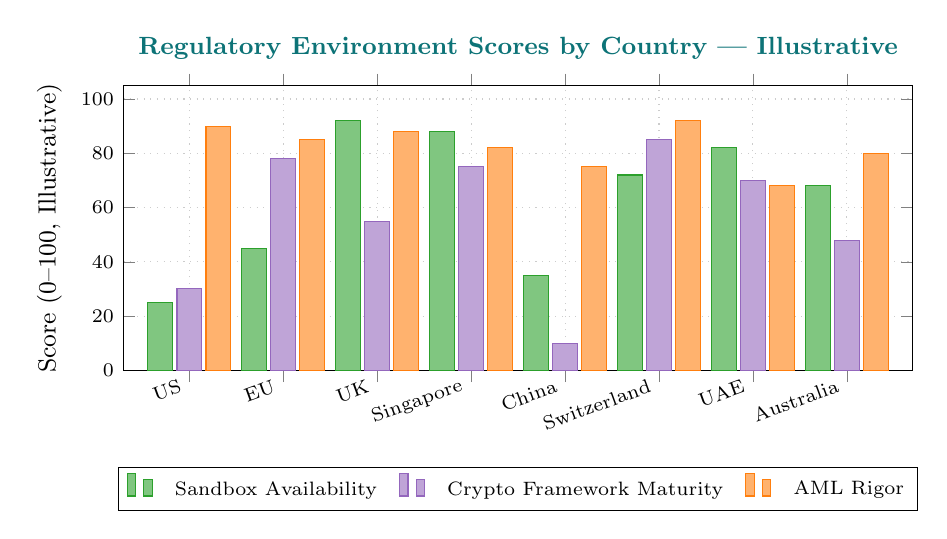
\begin{tikzpicture}
\begin{axis}[
  width=11.6cm, height=5.2cm,
  ybar=1.5pt,
  bar width=9pt,
  enlarge x limits=0.10,
  ylabel={\small Score (0--100, Illustrative)},
  ylabel style={font=\scriptsize},
  symbolic x coords={US, EU, UK, Singapore, China, Switzerland, UAE, Australia},
  xtick=data,
  xticklabel style={font=\scriptsize, rotate=20, anchor=east},
  ymin=0, ymax=105,
  ytick={0,20,40,60,80,100},
  yticklabel style={font=\scriptsize},
  legend style={font=\scriptsize, at={(0.5,-0.34)}, anchor=north,
                legend columns=3, column sep=6pt},
  legend cell align=left,
  grid=major,
  grid style={dotted,mlgray!40},
  title={\small\bfseries\textcolor{mlteal}{Regulatory Environment Scores by Country --- Illustrative}},
  title style={font=\small},
  clip=false,
]

% Sandbox availability (0-100)
\addplot[fill=mlgreen!60,draw=mlgreen] coordinates {
  (US,        25)
  (EU,        45)
  (UK,        92)
  (Singapore, 88)
  (China,     35)
  (Switzerland,72)
  (UAE,       82)
  (Australia, 68)
};

% Crypto framework maturity (0-100)
\addplot[fill=mlpurple!60,draw=mlpurple] coordinates {
  (US,        30)
  (EU,        78)
  (UK,        55)
  (Singapore, 75)
  (China,     10)
  (Switzerland,85)
  (UAE,       70)
  (Australia, 48)
};

% AML rigor (0-100)
\addplot[fill=mlorange!60,draw=mlorange] coordinates {
  (US,        90)
  (EU,        85)
  (UK,        88)
  (Singapore, 82)
  (China,     75)
  (Switzerland,92)
  (UAE,       68)
  (Australia, 80)
};

\legend{Sandbox Availability, Crypto Framework Maturity, AML Rigor}
\end{axis}
\end{tikzpicture}
\end{center}
\vspace{-0.4em}
{\tiny\textcolor{mlgray}{All scores are illustrative composites based on publicly available indices (Global Financial Centres Index, FATF evaluations, Cambridge Centre for Alternative Finance reports). Not official ratings.}}
\bottomnote{Slide 7/10 --- WHERE | Financial Technology -- MSc | University of Zurich | Spring 2026}
\end{frame}

% ============================================================
%  FRAME 8 -- IMPACT: TikZ diagram -- RegTech technology stack
%             layers (data -> processing -> analytics -> reporting)
% ============================================================
\begin{frame}{Impact: The RegTech Technology Stack}
\begin{center}
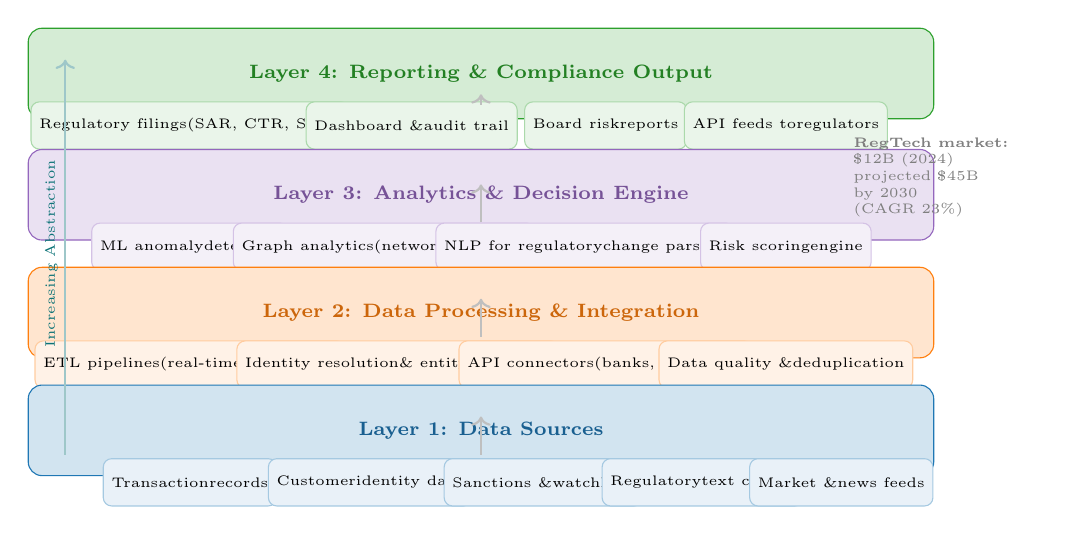
\begin{tikzpicture}[scale=0.88,
  layer/.style={rectangle,rounded corners=5pt,minimum width=11.5cm,
                minimum height=1.15cm,font=\scriptsize\bfseries,
                text centered},
  component/.style={rectangle,rounded corners=3pt,minimum height=0.6cm,
                    font=\tiny,text centered,inner sep=3pt},
  arr/.style={->,thick,draw=mlgray!50}
]

  % ---- Layer 4 (top): REPORTING & COMPLIANCE OUTPUT ------------
  \node[layer,fill=mlgreen!20,draw=mlgreen,text=mlgreen!80!black]
    (L4) at (0, 3.3) {Layer 4: Reporting \& Compliance Output};

  \node[component,fill=mlgreen!10,draw=mlgreen!40] at (-4.2,2.55)
    {Regulatory filings\\(SAR, CTR, STR)};
  \node[component,fill=mlgreen!10,draw=mlgreen!40] at (-1.0,2.55)
    {Dashboard \&\\audit trail};
  \node[component,fill=mlgreen!10,draw=mlgreen!40] at (1.8,2.55)
    {Board risk\\reports};
  \node[component,fill=mlgreen!10,draw=mlgreen!40] at (4.4,2.55)
    {API feeds to\\regulators};

  % ---- Layer 3: ANALYTICS & DECISION ENGINE --------------------
  \node[layer,fill=mlpurple!20,draw=mlpurple,text=mlpurple!80!black]
    (L3) at (0, 1.55) {Layer 3: Analytics \& Decision Engine};

  \node[component,fill=mlpurple!10,draw=mlpurple!40] at (-4.2,0.8)
    {ML anomaly\\detection};
  \node[component,fill=mlpurple!10,draw=mlpurple!40] at (-1.4,0.8)
    {Graph analytics\\(network analysis)};
  \node[component,fill=mlpurple!10,draw=mlpurple!40] at (1.5,0.8)
    {NLP for regulatory\\change parsing};
  \node[component,fill=mlpurple!10,draw=mlpurple!40] at (4.4,0.8)
    {Risk scoring\\engine};

  % ---- Layer 2: DATA PROCESSING & INTEGRATION ------------------
  \node[layer,fill=mlorange!20,draw=mlorange,text=mlorange!80!black]
    (L2) at (0, -0.15) {Layer 2: Data Processing \& Integration};

  \node[component,fill=mlorange!10,draw=mlorange!40] at (-4.2,-0.9)
    {ETL pipelines\\(real-time streaming)};
  \node[component,fill=mlorange!10,draw=mlorange!40] at (-1.2,-0.9)
    {Identity resolution\\\& entity matching};
  \node[component,fill=mlorange!10,draw=mlorange!40] at (1.8,-0.9)
    {API connectors\\(banks, registries)};
  \node[component,fill=mlorange!10,draw=mlorange!40] at (4.4,-0.9)
    {Data quality \&\\deduplication};

  % ---- Layer 1 (bottom): DATA SOURCES --------------------------
  \node[layer,fill=mlblue!20,draw=mlblue,text=mlblue!80!black]
    (L1) at (0, -1.85) {Layer 1: Data Sources};

  \node[component,fill=mlblue!10,draw=mlblue!40] at (-4.2,-2.6)
    {Transaction\\records};
  \node[component,fill=mlblue!10,draw=mlblue!40] at (-1.6,-2.6)
    {Customer\\identity data};
  \node[component,fill=mlblue!10,draw=mlblue!40] at (0.9,-2.6)
    {Sanctions \&\\watchlists};
  \node[component,fill=mlblue!10,draw=mlblue!40] at (3.2,-2.6)
    {Regulatory\\text corpus};
  \node[component,fill=mlblue!10,draw=mlblue!40] at (5.2,-2.6)
    {Market \&\\news feeds};

  % ---- Vertical arrows between layers -------------------------
  \draw[arr] (0,-2.2) -- (0,-1.65);
  \draw[arr] (0,-0.5) -- (0,0.05);
  \draw[arr] (0,1.15) -- (0,1.7);
  \draw[arr] (0,2.85) -- (0,3.0);

  % ---- Side annotations ---------------------------------------
  \node[font=\tiny,text=mlteal,align=center,rotate=90]
    at (-6.2,0.7) {Increasing Abstraction};
  \draw[mlteal!40,->,thick] (-6.0,-2.2) -- (-6.0,3.5);

  % Right-side market sizing
  \node[font=\tiny,text=mlgray,align=left,text width=2.5cm]
    at (6.8,1.8) {\textbf{RegTech market:}\\\$12B (2024)\\projected \$45B\\by 2030\\(CAGR 23\%)};

\end{tikzpicture}
\end{center}
\bottomnote{Slide 8/10 --- IMPACT | Financial Technology -- MSc | University of Zurich | Spring 2026}
\end{frame}

% ============================================================
%  FRAME 9 -- SO WHAT: Evaluation checklist --
%             5 questions for any regulatory framework
% ============================================================
\begin{frame}{So What? Five Questions to Evaluate Any Regulatory Framework}

\vspace{0.3em}
\begin{columns}[T]
\begin{column}{0.62\textwidth}

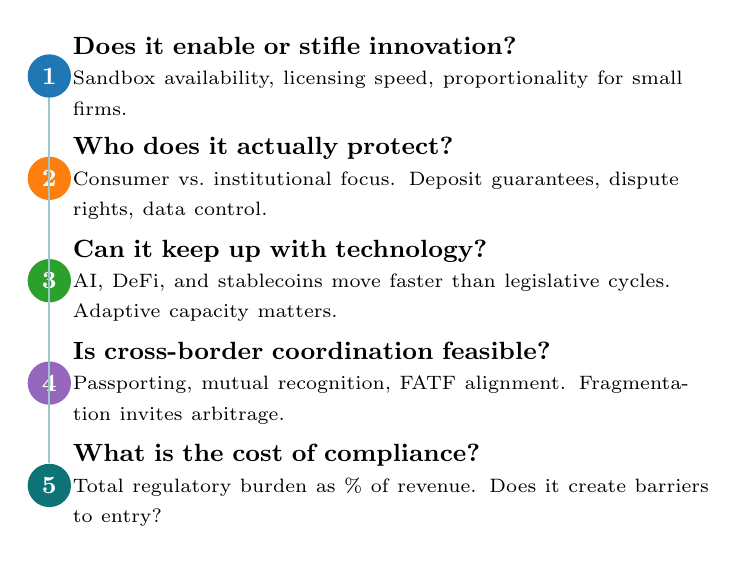
\begin{tikzpicture}[
  chk/.style={circle,minimum size=0.55cm,font=\small\bfseries,
              inner sep=0pt,text=white},
  lbl/.style={font=\small,text width=8.2cm,align=left}
]

% ---- Row 1 --------------------------------------------------
\node[chk,fill=mlblue]    (c1) at (0, 0)   {1};
\node[lbl] at (4.4, 0)
  {\textbf{Does it enable or stifle innovation?}\\
   {\scriptsize Sandbox availability, licensing speed, proportionality for small firms.}};

% ---- Row 2 --------------------------------------------------
\node[chk,fill=mlorange]  (c2) at (0,-1.3) {2};
\node[lbl] at (4.4,-1.3)
  {\textbf{Who does it actually protect?}\\
   {\scriptsize Consumer vs.\ institutional focus. Deposit guarantees, dispute rights, data control.}};

% ---- Row 3 --------------------------------------------------
\node[chk,fill=mlgreen]   (c3) at (0,-2.6) {3};
\node[lbl] at (4.4,-2.6)
  {\textbf{Can it keep up with technology?}\\
   {\scriptsize AI, DeFi, and stablecoins move faster than legislative cycles. Adaptive capacity matters.}};

% ---- Row 4 --------------------------------------------------
\node[chk,fill=mlpurple]  (c4) at (0,-3.9) {4};
\node[lbl] at (4.4,-3.9)
  {\textbf{Is cross-border coordination feasible?}\\
   {\scriptsize Passporting, mutual recognition, FATF alignment. Fragmentation invites arbitrage.}};

% ---- Row 5 --------------------------------------------------
\node[chk,fill=mlteal]    (c5) at (0,-5.2) {5};
\node[lbl] at (4.4,-5.2)
  {\textbf{What is the cost of compliance?}\\
   {\scriptsize Total regulatory burden as \% of revenue. Does it create barriers to entry?}};

% Vertical connector line
\draw[mlteal!40,thick] (0,-0.28) -- (0,-4.92);

\end{tikzpicture}

\end{column}
\begin{column}{0.34\textwidth}
\vspace{0.2em}
\begin{block}{When to Use This}
\scriptsize
\begin{itemize}
  \item Evaluating a new market for fintech expansion
  \item Comparing regulatory regimes for a policy paper
  \item Assessing RegTech vendor claims
  \item Preparing for the regulation case study workshop
\end{itemize}
\end{block}
\vspace{0.2em}
\begin{exampleblock}{Worked Example}
\scriptsize
\textbf{UK FCA Sandbox (2016--)}\\
Innovation: pioneer, 800+ firms tested\\
Protection: consumer safeguards maintained\\
Adaptiveness: iterates annually\\
Cross-border: GFIN co-operation\\
Cost: reduced via sandbox exemptions
\end{exampleblock}
\end{column}
\end{columns}

\bottomnote{Slide 9/10 --- SO WHAT | Financial Technology -- MSc | University of Zurich | Spring 2026}
\end{frame}

% ============================================================
%  FRAME 10 -- ACT: Activity prompt + next lecture preview
%              (L05: Personal Finance and Wealth Management)
% ============================================================
\begin{frame}{Act: Analyse a Regulatory Framework End to End}

\begin{columns}[T]
\begin{column}{0.56\textwidth}
\begin{block}{Your Task (15 Minutes)}
\scriptsize
Choose \textbf{one jurisdiction} from the table on Slide 3 (or your home country). Reconstruct its fintech regulatory environment:
\begin{enumerate}\scriptsize
  \item \textbf{Licensing:} What license does a payments fintech need? How long does it take?
  \item \textbf{AML/KYC:} Which authority supervises? What are the main obligations?
  \item \textbf{Crypto:} Is there a framework? Banned, tolerated, or fully regulated?
  \item \textbf{Sandbox:} Does one exist? How many firms have graduated?
  \item \textbf{Five-question test:} Apply the checklist from Slide 9. Score each dimension 1--5.
\end{enumerate}
\end{block}
\vspace{0.2em}
\begin{exampleblock}{Reflection Prompt}
\scriptsize
If you were the \textbf{founder} of a cross-border payments startup, which jurisdiction would you incorporate in first -- and why? If you were the \textbf{regulator}, what single change would most improve fintech innovation without compromising consumer protection?
\end{exampleblock}
\end{column}
\begin{column}{0.40\textwidth}
\begin{exampleblock}{Discussion Starter}
\scriptsize
\begin{itemize}
  \item Is the EU's ``regulate first'' approach (MiCA, DORA, AI Act) a competitive advantage or a burden?
  \item Can RegTech truly replace human compliance officers, or does it just add a layer?
  \item Why do some countries ban crypto trading but develop CBDCs?
\end{itemize}
\end{exampleblock}
\vspace{0.2em}
\begin{alertblock}{Next Lecture --- L05}
\scriptsize \textbf{Personal Finance and Wealth Management}\\
From robo-advisors to AI-driven financial planning: how technology is democratising wealth management.\\[3pt]
\textit{Prepare: check the fee structure of one robo-advisor (e.g., Betterment, Wealthfront, or True Wealth).}
\end{alertblock}
\end{column}
\end{columns}

\bottomnote{Slide 10/10 --- ACT | Financial Technology -- MSc | University of Zurich | Spring 2026}
\end{frame}

% ============================================================
\end{document}
% ============================================================
